\section{Ableitung, Integration}

\begin{itemize}
 	\item \textbf{Summenregel} $(f(x)+g(x))' = f'(x) + g'(x)$
    \item \textbf{Produktregel} $(f(x)\cdot g(x))' = f'(x)g(x) + f(x)g'(x)$
    \item \textbf{Quotientenregel} $\left(\frac{f(x)}{g(x)}\right)' = \frac{f'(x)g(x) - f(x)g'(x)}{g^2(x)}(g\neq 0)$
    \item \textbf{Kettenregel} $(f(g(x)))' = (f\circ g)' = f'(g(x))g'(x)$
\end{itemize}

\begin{itemize}
  \item \textbf{Partielle Integration:} $\int_a^b f'(x)\cdot g(x)dx = \left[f(x)g(x)\right]_a^b - \int_a^b f(x)g'(x)$
  \item \textbf{Substitution:} $\int_{\phi(a)}^{\phi(b)} f(x)dx = \int_a^b f(\phi(t))\phi '(t) dt$
  \item \textbf{$a+c, b+c \in I$} $\int_a^b f(t+c)dt = \int_{a+c}^{b+c} f(x)dx$
  \item \textbf{$ca,cb\in I$: } $\int_a^b f(ct)dt = \frac{1}{c}f(x)dx$
  \item \textbf{Logarithmus: }\;$\int\frac{f'(t)}{f(t)}dt = \log(|f(x)|)$, bzw. $\int_a^b\frac{f'(t)}{f(t)}dt = \log(f(|b|)) - \log(f(|a|))$
\end{itemize}

\section{Nützlich}

\textbf{Erwartungswert Stuff}



Median berechnen: Die Vertilungsfunktion muss $= 0.5$ sein. Also sei $F_X(x) = 0.5$, dann ist $x$ der Median.\\

Falls $Y = g(X)$, dann $F_Y(x) = F_X(g^{-1}(x))$\\

Falls $X_i \sim \text{Poi}(\lambda)$, dann $S_n \sim \text{Poi}(n \cdot \lambda)$
\\

Falls $X_i \sim \mathcal{N}(\mu, \sigma^2)$, dann $$\overline{X_n} \sim \mathcal{N}(\mu, \frac{\sigma^2}{n}),\quad\frac{\overline{X_n}-\mu}{\sigma / \sqrt{n}} \sim \mathcal{N}(0, 1)$$

$$
	\mathbb{E}[X] = \int_{-\infty}^\infty x \cdot f_X(x)\ dx,\quad
	\mathbb{E}[X^k] = \int_{-\infty}^\infty x^k \cdot f_X(x)\ dx\quad
	\text{(vgl. Satz 4.3)}
$$

Die Likelihoodmethode ist eigentlich die gemeinsame Dichte (Produkt falls unabhängig).\\

Stichprobenmittel: $$\overline{X}_n = \frac{1}{n	}\sum_{i=1}^nX_i$$

Stichprobenvarianz: $$S^2 = \frac{1}{n-1}\sum^n_{i=1}\left(X_i-\overline{X}_n\right)^2$$

Das Stichprobenmittel und die Stichprobenvarianz werden oft als Schätzer in Kofidenzbereichen verwendet.\\

\section{Schätzer Rezepte}

\subsection{Maximum Likelihood Schätzer}

\begin{itemize}
	\item Likehood-Funktion $L$ bestimmen
	\item Falls Zufallsvariablen i.i.d., dann $\log L$ bestimmen
	\item $\log L$ (oder $L$) maximieren: ableiten von $\log L$ (oder $L$) und gleich $0$ setzen.
	\item $\Rightarrow$ Funktion, die Parameter schätzt
\end{itemize}

\subsection{Momentenschätzer mit zentralen/rohen Momenten}

$k$-tes \textbf{rohes} Moment: $\E[X^k]$

$k$-tes empirisches \textasciitilde: $\frac{1}{n}\sum_{i=1}^nx_i^k$\\

$k$-tes \textbf{zentrales} Moment: $\E[(X - \E[X])^k]$

1. theoretisches \textasciitilde = $\mathbb{E}[X]$, 2. theoretisches \textasciitilde = $\text{Var}[X]$)

1. empirisches \textasciitilde = $\overline{X}$, 2. emprisches \textasciitilde = $\frac{1}{n}\sum_{i=1}^n(X_i-\overline{X})^2$, $k$-tes empirisches \textasciitilde: $\frac{1}{n}\sum_{i=1}^n(X_i-\overline{X})^k$

\subsubsection{Rezept}

\begin{itemize}
	\item Verteilung bestimmen, $\vartheta$ bestimmen ($k$ argumente)
	\item Die ersten $k$ theoretische zentrale/rohe Momente bestimmen
	\item Gleichstellen mit empirischen zentralen/rohen Momenten
	\item $\Rightarrow$ Funktion, die Parameter schätzt.
\end{itemize}

\section{p-Wert}

Beispiel: Hintergrundfarbe einer Webseite ändern und schauen, ob sich die Besuchsdauer von Nutzern verändern. $$\mu = 20$$

\begin{itemize}
	\item Nullhypothese $H_0$: $\mu = 20$ nach der Änderung\\Alternative $H_A$: $\mu > 20$ nach der Änderung
	\item Signifikanzniveau: $\alpha = 0.05$
	\item Stichprobe: $n=100$, $\overline{X} = 25$, ($\sigma$)
	\item p-Wert: $P[\overline{X} \geq 25 \mid H_0 \text{ ist wahr}]$
	\item Falls p-Wert $< \alpha$: $H_0$ verwerfen (und $H_A$ akzeptieren)\\Falls p-Wert $\geq \alpha$: $H_0$ nicht verwerfen (keine Aussage)
\end{itemize}

Der p-Wert ist \textbf{nicht} $P[H_0 \text{ ist wahr} \mid \text{Stichprobe}]$

\section{Tests}

Zusammenhänge $\alpha$ (Signifikanzniveau), Fehler 1. Art, $\beta$ (Macht), Fehler 2. Art ($1-\beta$)

\begin{itemize}
	\item $\alpha$ grösser $\iff$ Fehler 1. Art grösser $\iff$ Fehler 2. Art kleiner $\iff$ Macht grösser
	\item $\alpha$ kleiner $\iff$ Fehler 1. Art kleiner $\iff$ Fehler 2. Art grösser $\iff$ Macht kleiner
\end{itemize}

\textbf{Achtung:} Bei kleinen Datenmengen kann eine Normalverteilungsapproximation ungenau werden. Deshalb immer diskrete Werte verwenden.

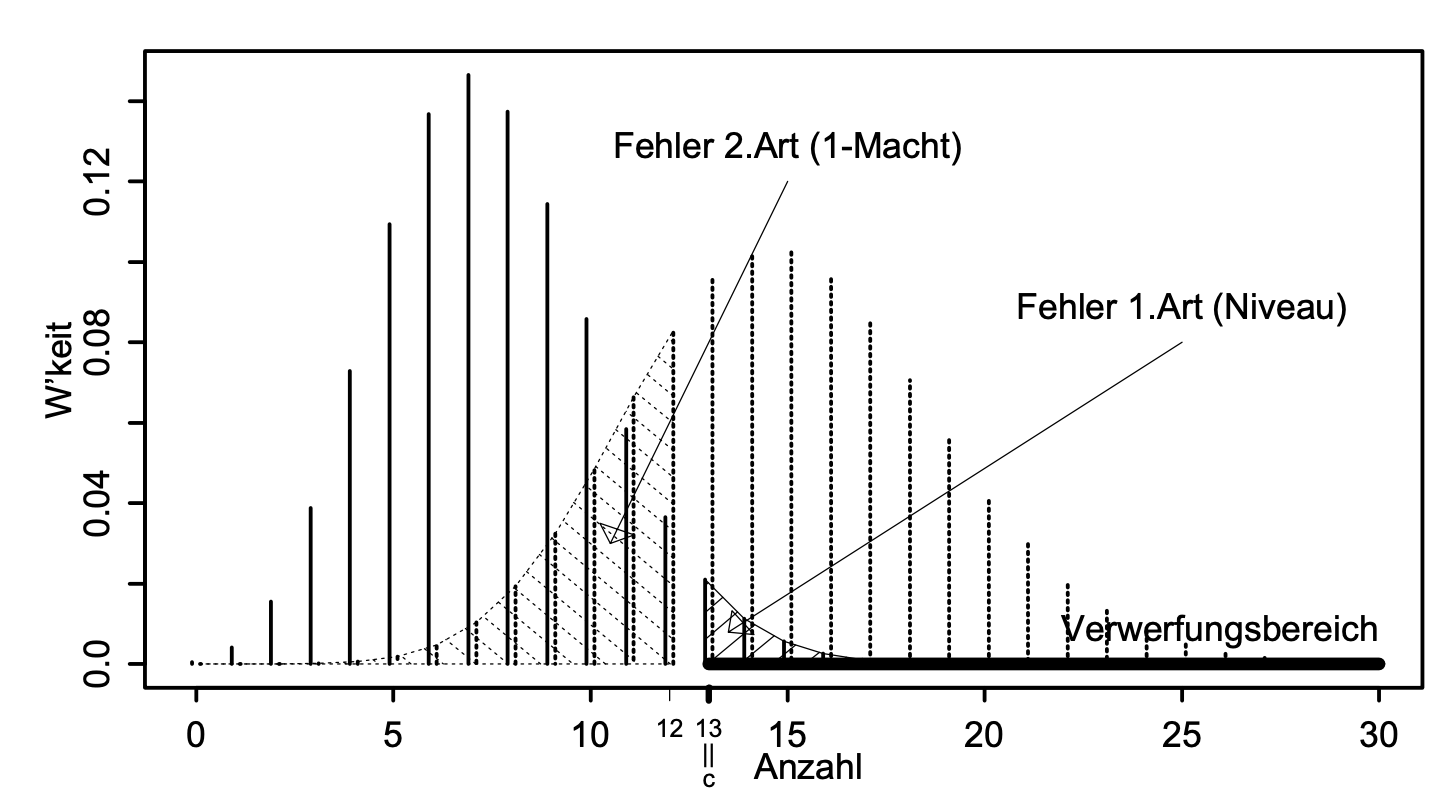
\includegraphics[width=.8\textwidth]{images/normal.png}

\subsection{Begriffe}

Modell: z.B. Unter $P_\varphi$ sind die $X_i$ i.i.d. $\sim\text{Poi}(\lambda)$, $i=1, ..., 6$, $\lambda$ unbekannt.

Teststatistik: Hilfsfunktion bei statistischen Tests. Kann zum Beispiel mittels Likelihood-Quotienten-Vorgehen gefunden werden.\\

\textbf{Punkte}; Beispiel jeweils in Klammern:
\begin{itemize}
	 \item Modell (\textit{Unter $P_\vartheta$ sind die $X_i$ i.i.d. $\sim$ Poi...})
	 \item Nullhypothese (\textit{$H_0: p = ...$})
	 \item Alternativhypothese (\textit{$H_A: p < ...$})
	 \item Teststatistik  (\textit{$T= <R>$ also Likelihood-Quotienten verwenden})
	 \item Verteilung der Teststatistik unter der Nullhypothese (\textit{$H_0: T \sim Bin...$})
	 \item Verwerfungsbereich ($K = [a, b]$, $P_{\vartheta_0}[T\in K] \leq 5\%...$)
	 \item beobachteter Wert der Teststatistik ($t=T(\omega)=6$)
	 \item Testentscheid (\textit{Nullhypothese wird nicht verworfen...})
	 \item eventuell $p$-Wert
\end{itemize}

\textbf{Wichtig:}

Falls beobachtetes Ergebnis im Verwerfungsbereich: $H_0$ wird abgelehnt, $H_A$ wird angenommen.

Falls beobachtetes Ergebnis nicht im Verwerfungsbereich: $H_0$ wird nicht abgelehnt (keine Aussage über Annahme!), keine Aussage über $H_A$\\

\textbf{$p$-Wert}: kleinstes Niveau, auf dem der Test die Nullhypothese noch verwirft.\\

Auch: Falls $H_0: p = 123$, $H_A: p < 123$ Mit Statistik $P_{H_0}[T\leq \text{Beobachteter Wert}]$. p-Wert ist so wie die Signifikanz des Testresultats.\\

A small p-value (typically $\leq 0.05$) indicates strong evidence against the null hypothesis, so you reject the null hypothesis.\\

A large p-value ($> 0.05$) indicates weak evidence against the null hypothesis, so you fail to reject the null hypothesis.

\section{Beispiel Teststatistik mit Likelihood-Quotienten finden}

$X_i \sim \text{Poi}(\lambda)$ 

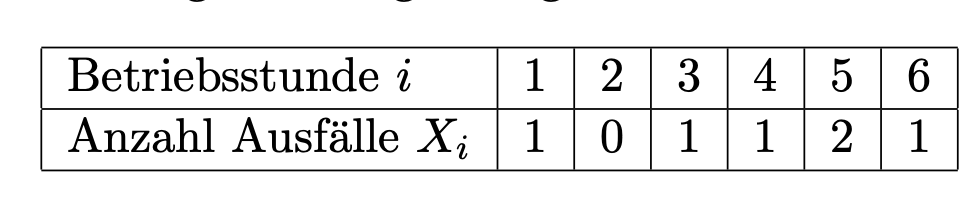
\includegraphics[width=.4\textwidth]{images/likelihood1}

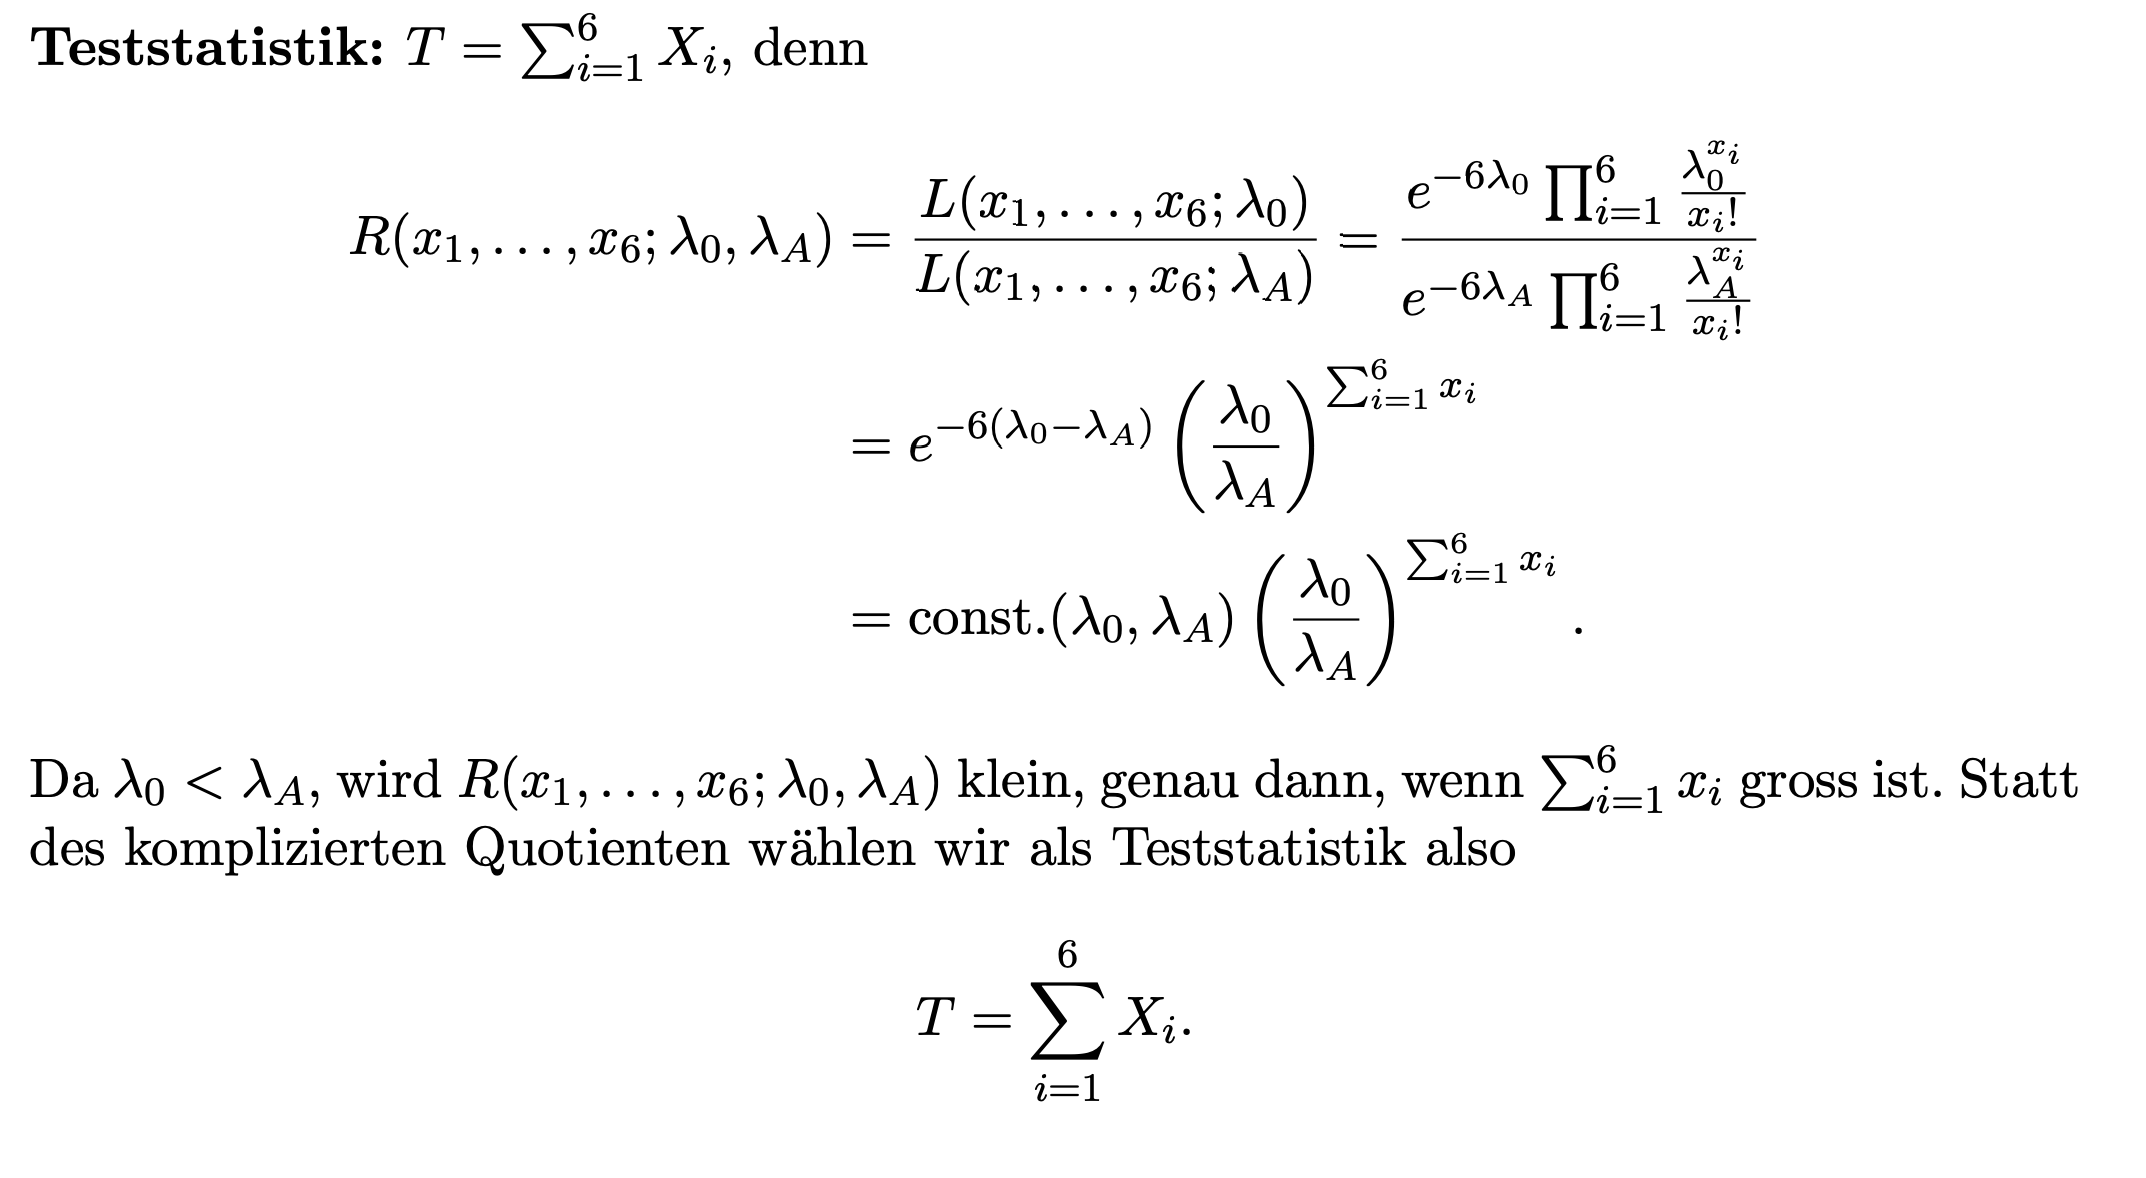
\includegraphics[width=\textwidth]{images/likelihood2}

\section{Konfidenzintervall berechnen}

\begin{itemize}
	\item Gegeben: Teststatistik $T$.
	\item Schätze $\vartheta$ mit einem Schätzer. Zum Beispiel $\mu$: Stichprobenmittel oder $\sigma$: Stichprobenvarianz.
	\item Setze den geschätzten Wert von $\vartheta$ in $T$ ein und bestimme die Verteilung. Achtung: Die Zufallsvariable ist frei. 
	\item Konfidenzintervall mit Niveau $1-\alpha$: Bereich in der neuen Verteilung, die die Fläche $1-\alpha$ hat. ACHTUNG: Bereich soll als Bereich der Zufallsvariable angegeben sein, bevor sie in die Teststatistik eingeben wird, sodass sie im Niveaubereich liegt.
\end{itemize}












































